\documentclass[10pt,xcolor=dvipsnames,serif,professionalfont]{beamer} %
\input{beamerpalatino}
\graphicspath{{../images/}}

\title[Multilevel Regression]{Multilevel Regression}
\author[Andrews]{Mark Andrews}
\date{Sept 14, 2016}

\DeclareSymbolFont{legacymaths}{OT1}{cmr}{m}{n}
\DeclareMathAccent{\dot}     {\mathalpha}{legacymaths}{95}
\DeclareMathAccent{\bar}     {\mathalpha}{legacymaths}{22}
\DeclareMathAccent{\tilde}     {\mathalpha}{legacymaths}{126}


\begin{document}
{
\begin{frame}
   \titlepage
\end{frame}
}

\section{Multiple Levels of Data}
\begin{frame}
\vspace{-1.5\baselineskip}
\begin{center}
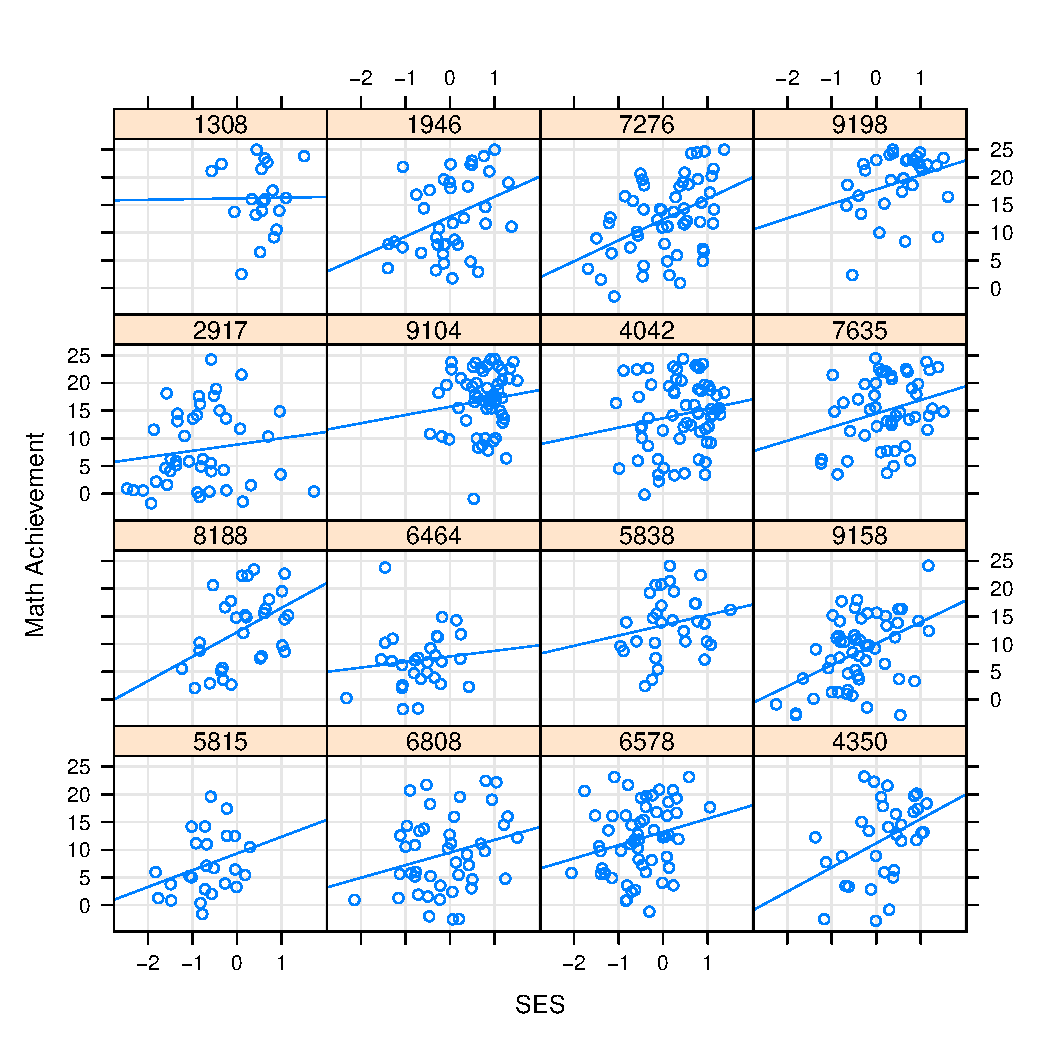
\includegraphics[width=.8\textwidth]{figs/mlplot.pdf}
\end{center}
\end{frame}

\begin{frame}
\frametitle{Example: Multilevel model for reaction times}
\begin{itemize}
\item Consider we have reaction time data from $J$ subjects, 
\[\{x_{j1}, x_{j2}, x_{j3} \ldots x_{jn_j}\}_{j=1}^J.\]
\item A simple multilevel model for this data might be:
\begin{align*}
x_{ji} &\sim N(\mu_j,\sigma^2),\quad\text{for $i \in \{1\ldots n_j\}$},\\
\mu_j &\sim N(\theta,\tau^2), \quad\text{for $j \in \{1 \ldots J\}$}.
\end{align*}
\item In words, each $x_{ji}$ is drawn from a Gaussian with mean $\mu_j$ and variance $\sigma^2$, and each $\mu_j$ is drawn from a Gaussian with mean $\theta$ and variance $\tau^2$.
\end{itemize}
\end{frame}


\begin{frame}
\frametitle{Example: Multilevel model for reaction times}
\begin{itemize}
\item We can re-write $x_{ji} \sim N(\mu_j,\sigma^2)$ as 
\[ x_{ji} = \mu_j + \epsilon_{ji},\quad \epsilon_{ji} \sim N(0,\sigma^2).\]
\item We can re-write $\mu_j\sim N(\theta,\tau^2)$ as 
\[ \mu_j = \theta + \eta_j, \quad \eta_{j} \sim N(0,\tau^2).\]
\item The multilevel model can be re-written 
\[ x_{ji} = \theta + \eta_j + \epsilon_{ji}\quad \epsilon_{ji} \sim N(0,\sigma^2), \eta_{j} \sim N(0,\tau^2).\]
\item This is often termed a \emph{random-effects} model.
\end{itemize}
\end{frame}

\begin{frame}
\frametitle{Example: Multilevel model for reaction times}
\begin{itemize}
\item In the model just described, there are three unknowns: $\theta$, $\sigma^2$ and $\tau^2$.
\item Model estimation (fitting) estimates values for these variables.
\item The variable $\theta$ denotes the global average reaction time.
\item The variable $\sigma^2$ denotes the variance within any given subject.
\item The variable $\tau^2$ denotes the variance across subjects.
\end{itemize}
\end{frame}

\begin{frame}
\frametitle{Example: Multilevel model for reaction times}
\begin{itemize}
\item In the model just described, $\theta$ tells us the global average.
\item The variance $\tau^2$ tells us how much any given subject's average varies about $\theta$.
\item For example, 95\% and 99\% of the averages for individual subjects,  will be in the ranges
\[\theta \pm 1.96 \times \tau,\quad  \theta \pm 2.56 \times \tau,\]
respectively.
\item Likewise, 95\% and 99\% of any given subject's reaction times, i.e. $x_{ji}$, will be in the ranges
\[\theta + \eta_j   \pm 1.96 \times \sigma,\quad \theta + \eta_j  \pm 2.56 \times \sigma.\]
\end{itemize}
\end{frame}


\begin{frame}[fragile]
\frametitle{Example: Multilevel model for reaction times}
\begin{itemize}
\item A model, such as the previous one, would be specified as follows in the \texttt{lmer} program in R:
\begin{center}
\begin{verbatim}
lmer(latency ~ 1 + (1|subject))
\end{verbatim}
\end{center}
where \texttt{latency} is reaction time, and \texttt{subject} is a categorical variable that indicates the identity of the subject.
\item In other words, here we are saying that reaction time is modelled as a variation around a global average plus an individual average.
\end{itemize}
\end{frame}


\begin{frame}
\frametitle{Example: Multiple drivers, multiple cars}
\begin{itemize}
\item Let's say we want to measure the mpg of a given model of car (e.g. a Porsche 911).
\item Because any one car could vary from others of the same model, we have $K$ different examples of this model of car.
\item Likewise, because any one driver could affect the recorded mpg of the car he drives, we have $J$ different drivers. 
\item We get each of the J drivers to drive each of the K cars, and record the mpg as 
\[y_{jk} = \text{mpg for driver $j$, car $k$}.\]
\end{itemize}
\end{frame}


\begin{frame}
\frametitle{Example: Multiple drivers, multiple cars}
\begin{itemize}
\item A multilevel model for this mpg experiment could be
\begin{align*}
y_{jk} &\sim N(\mu_{j} + \nu_k,\sigma^2),\\
\mu_{j} &\sim N(\phi,\tau^2)\\
\nu_{k} &\sim N(\psi,\upsilon^2)
\end{align*}
which would work out as 
\[y_{jk} = \underbrace{\theta}_{\phi + \psi} + \eta_j + \zeta_k + \epsilon_{jk},\]
with 
\[\eta_j \sim N(0,\tau^2),~ \zeta_k \sim N(0,\upsilon^2),~ \epsilon_{jk} \sim N(0,\sigma^2).\]
\end{itemize}
\end{frame}


\begin{frame}
\frametitle{Example: Multiple drivers, multiple cars}
\begin{itemize}
\item In this example, we have three sources of variation 
\[y_{jk} = \theta + \underbrace{\eta_j}_{\text{\tiny within driver}} + \underbrace{\zeta_k}_{\text{\tiny within car}} + \underbrace{\epsilon_{jk}}_{\text{\tiny within trial}},\]
where $\tau^2$ gives the within driver variance, $\upsilon^2$ gives the within car variation, and $\sigma^2$ gives within trial variation.
\item The variable $\theta$ provides the average mpg for the car model (i.e. the Porsche 911)
\item \emph{Your mileage may vary}: The variables $\tau^2$, $\upsilon^2$ and $\sigma^2$ provide measures of the relative variation across in mpg drivers, cars and trials, respectively.
\end{itemize}
\end{frame}


\begin{frame}[fragile]
\frametitle{Example: Multiple drivers, multiple cars}
\begin{itemize}
\item The mpg model would be specified as follows in the \texttt{lmer}:
\begin{center}
\begin{verbatim}
lmer(mpg ~ 1 + (1|driver) + (1|car))
\end{verbatim}
\end{center}
where \texttt{mpg} is continuous variable, and \texttt{driver} and \texttt{car} are categorical variables that indicate the identity of the driver and car, respectively.
\end{itemize}
\end{frame}

\begin{frame}
\frametitle{Example: Mathematical achievement and socioeconomic status}
\begin{itemize}
\item In this problem, we have $J$ schools. Within each school, we have $n_j$ students. 
\item For student $i$ in school $j$, their ses score is $x_{ji}$ and their mathematical achievemnt score is $y_{ji}$.
\item A multilevel model for this data is 
\begin{align*}
y_{ji} &\sim N(\alpha_{j} + \beta_j x_{ji},\sigma^2),\\
\alpha_j &\sim N(a,\tau_a^2),\\
\beta_j &\sim N(b,\tau_b^2).
\end{align*}
\end{itemize}
\end{frame}


\begin{frame}
\frametitle{Example: Mathematical achievement and socioeconomic status}
\begin{itemize}
\item The model
\begin{align*}
y_{ji} &\sim N(\alpha_{j} + \beta_j x_{ji},\sigma^2),\\
\alpha_j &\sim N(a,\tau_a^2),\\
\beta_j &\sim N(b,\tau_b^2),
\end{align*}
can be re-written
\[y_{ji} = a + bx_{ji} + \eta_j + \zeta_j x_{ji} + \epsilon_{ji},\]
where 
\[\eta_j \sim N(0,\tau_a^2),~ \zeta_j \sim N(0,\tau_b^2),~ \epsilon_j \sim N(0,\sigma^2).\]
\end{itemize}
\end{frame}

\begin{frame}
\frametitle{Example: Mathematical achievement and socioeconomic status}
\begin{itemize}
\item We can look at this model as 
\[y_{ji} = \underbrace{a + bx_{ji}}_{\text{\tiny general model}} + \underbrace{\eta_j + \zeta_j x_{ji}}_{\text{\tiny school-level model}} + \epsilon_{ji}.\]
\item For any given school, the model can be viewed as 
\[y_{ji} = \underbrace{(a + \eta_j)}_{\text{ $\alpha_j$}} + \underbrace{(b + \zeta_j)}_{\text{ $\beta_j$}} x_{ji} + \epsilon_{ji}.\]
\item In other words, any given school's regression model is a variation on a general regression model.
\end{itemize}
\end{frame}

\begin{frame}
\frametitle{Example: Mathematical achievement and socioeconomic status}
\begin{itemize}
\item In the model just described, $a$ and $b$ are the general regression coefficients. 
\item The variance $\tau_a^2$ tells us how much variation in the intercept term there is across schools. The variance $\tau_b^2$ tells us how much variation in the slope term there is across schools. 
\item For example, 95\% and 99\% of the intercepts for individual schools will be in the ranges
\[a \pm 1.96 \times \tau_a,\quad  a \pm 2.56 \times \tau_a,\]
respectively. Likewise, 95\% and 99\% of the slope terms for schools will be in the ranges
\[ b \pm 1.96 \times \tau_b,\quad b  \pm 2.56 \times \tau_b.\]
\end{itemize}
\end{frame}

\begin{frame}[fragile]
\frametitle{Example: Mathematical achievement and socioeconomic status}
\begin{itemize}
\item The ses regression model would be specified as follows in the \texttt{lmer}:
\begin{center}
\begin{verbatim}
lmer(math ~ 1 + ses + (1|school) + (0 + ses|school))
\end{verbatim}
\end{center}
where \texttt{math} is continuous variable, and \texttt{school} is a categorical variable that indicates the identity of the school\footnote{Writing \texttt{(1 + ses|school)} would imply correlated slopes and intercepts.}
\end{itemize}
\end{frame}



\begin{frame}
\frametitle{Why multilevel models?}
\begin{itemize}
\item When data occurs in groups, multilevel models should always be considered.
\item Multilevel models provide a macro/micro perspective on the data: The show the general pattern across all groups, and show how each individual group varies about this general pattern.
\item By appropriately indentifying different sources of variation, the general patterns in the data are more accurately inferred.
\item Even estimates for an individual group are improved by a process of \emph{strength-sharing}. In other words, knowing the general pattern in the data facilitates the inference of the patterns for individual 
\end{itemize}
\end{frame}



\end{document}

